% options:
% thesis=B bachelor's thesis
% thesis=M master's thesis
% czech thesis in Czech language
% slovak thesis in Slovak language
% english thesis in English language
% hidelinks remove colour boxes around hyperlinks

\documentclass[thesis=B,czech]{FITthesis}[2012/06/26]

\usepackage[utf8]{inputenc} % LaTeX source encoded as UTF-8

\usepackage{graphicx} %graphics files inclusion
% \usepackage{amsmath} %advanced maths
% \usepackage{amssymb} %additional math symbols
\usepackage{dirtree} %directory tree visualisation

\usepackage{listings}
\usepackage{placeins}


% % list of acronyms
\usepackage[acronym,nonumberlist,toc,numberedsection=autolabel]{glossaries}
% \iflanguage{czech}{\renewcommand*{\acronymname}{Seznam pou{\v z}it{\' y}ch zkratek}}{}
\makeglossaries

\newcommand{\tg}{\mathop{\mathrm{tg}}} %cesky tangens
\newcommand{\cotg}{\mathop{\mathrm{cotg}}} %cesky cotangens

% % % % % % % % % % % % % % % % % % % % % % % % % % % % % % 
% ODTUD DAL VSE ZMENTE
% % % % % % % % % % % % % % % % % % % % % % % % % % % % % % 

\department{Katedra Softwarového Inženýrství}
\title{Formát a~konverzní nástroje pro video z~webu na mobilních zařízeních}
\authorGN{Jan} %(křestní) jméno (jména) autora
\authorFN{Štěpanovský} %příjmení autora
\authorWithDegrees{Jan Štěpanovský} %jméno autora včetně současných akademických titulů
\supervisor{Ing. Pavel Štěpán}

\acknowledgements{
Chtěl bych poděkovat především vedoucímu práce Ing. Pavlovi Štěpánovi za vstřícnost a~důvěru při vytváření tohoto vlastního tématu. Dále bych chtěl poděkovat všem kolegům a~klientům, kteří mi poskytli prostor tento formát vyzkoušet. 

Dále bych chtěl poděkovat svým rodičům, bez kterých bych neměl možnost tuto práci napsat.
}

\abstractCS{V této práci je zdokumentován postup vytváření animací ve webových prohlížečích v~optimalizovaném formátu. Je zde popsáno vše od výzkumu, až po řešené přiklady použtí a~srovnání s~existujícími postupy. Z~této práce a~jejich výsledků mohou čerpat weboví vývojáři při vytváření animací na svých stránkách. }

\abstractEN{This work captures progress of creating animation in custom format in web interface. It contains everything from research to working examples with comparsion to current solutions. Web developers can use this work and its results as a~resource for creating animations on their web pages.  }

\placeForDeclarationOfAuthenticity{V~Praze}
\declarationOfAuthenticityOption{4} %volba Prohlášení (číslo 1-6)
\keywordsCS{javascript, python, html5, canvas, animace, formát}
\keywordsEN{javascript, python, html5, canvas, animation, format}

\begin{document}

% \newacronym{CVUT}{{\v C}VUT}{{\v C}esk{\' e} vysok{\' e} u{\v c}en{\' i} technick{\' e} v~Praze}
% \newacronym{FIT}{FIT}{Fakulta informa{\v c}n{\' i}ch technologi{\' i}}

\begin{introduction}

Internetové technologie slouží mimo jiné jako reklamní formát, který používají firmy a~jednotlivci k~prezentaci své značky. V~dnešní době už kromě hezké grafiky lze internetovou prezentaci oživit i~animací.

Pojmem animace se myslí jakýkoliv pohyblivý obrázek, který se na stránkách nyní řeší pomocí různých technologií. Při reálném použití se vyskytují určité nevýhody. Mezi ně patří například podpora v~mobilních prohlížečích, datová velikost nebo kvalita barev u~zobrazení. 

Současné možnosti technologie HTML5 se rozšířily o~element Canvas, který slouží k~vykreslování různých objektů a~bitmap pomocí technologie Javascript. Je možné navrhnout speciální animační formát, který by využíval tyto nativní technologie.

K napsání této bakalářské práce mě inspiroval článek\cite{appleWebsite} o~stránkách firmy Apple\cite{apple}, která tento jiný formát použila\cite{engadget} při představení nového produktu.

V této práci se věnuji jednoduchým animacím, kde se na jakkoli velké ploše mění pouze část stránky bez ztráty kvality ilustrace při animaci. Jedná se například o~animaci v~logu stránky nebo záznam používání webové aplikace. V~těchto případech se nám hodí snadná ovladatelnost a~budeme klást požadavky na spuštění až po provedení nějaké události.


\section{Struktura práce}

Kapitoly práce jsou rozvrženy tak, aby odpovídaly i~skutečnému pořadí prováděných úkolů. V~první kapitole je uveden cíl práce tak, aby bylo lépe poznat, na co je třeba se v~dalších kapitolách zaměřit a~o co se pokusit v~implementaci. 

V druhé kapitole je proveden průzkum současných možných řešení a~definování možné alternativní formy pro vytvoření animace, která by stále měla prostor mezi současnou technologií.

Třetí kapitola se zabývá analýzou potřeb a~dalších požadavků pro nový animační formát. Jelikož zadáním práce je vydefinování alternativního formátu, bude potřeba vytvořit jak generátor animace, tak přehrávač.

Ve čtvrté kapitole na základě analýzy definuji formát a~popíšu algoritmus zakódování a~přehrávání. 

V dalších kapitolách se věnuji návrhu a~implementace obou částí projektu, tedy návrh a~implementace generátoru a~přehrávače ve webovém rozhraní. 

V poslední deváté kapitole jsou popsány praktická využití formátu a~zhodnocení oproti současným možnostem.


\end{introduction}

\chapter{Cíl práce}

Cílem práce je vyzkoušet všechna stávající řešení, která umožňují animaci na stránkách a~navrhnout a~implementovat řešení, které bude  splňovat následující podmínky: 
\begin{itemize}
  \item Ovladatelnost přes skriptovací jazyk Javascript
  \item Široká podpora od mobilních zařízení po Internet Explorer
  \item Snadná implementace pro vstupní formáty GIF, MP4 (H.264)
  \item Optimalizace výstupu pro zajištění co nejmenší datové velikosti
\end{itemize}

Je potřeba navrhnout a~popsat algoritmus, který by dokázal konkurovat stávájícím řešením právě díky použití nativních technologií moderních webových prohlížečů (HTML5, Canvas). 

V této práci budou zdokumentovány všechny důležité kroky jako analýza, návrh, realizace, testování, příklady se zhodnocením a~výsledky. 
\chapter{Dostupná řešení}


Cílem této kapitoly  je provést průzkum dostupných řešení pro animaci na stránkách s~cílem zmapování dostupné funkcionality. U~různých formátů se sledují tyto vlastnosti:

\begin{itemize}
\item Použitelnost na mobilních zařízení
\item Kvalita a~plynulost animace
\item Datová velikost animace
\end{itemize}

Použitelnost na mobilních zařízení se zkoušela na Apple iPhone 6\cite{iphone5} a~Samsung Galaxy Trend Mini \cite{samsung}.


\section{Adobe Flash}

Adobe Flash\cite{flash} je komplexní nástroj, se kterým lze vytvářet velké aplikace v~prostředí webových prohlížečů. Má vlastní nástroj pro vytváření projektů Adobe Flash MX (obrázek \ref{fig:flash-ui}), ve kterém se celý program vytváří a~testuje. Na webovou stránku se umístí  speciální HTML\cite{html5video} objekt, který tento program použije pro vykreslení objektu.


\begin{figure}[h]
\centering
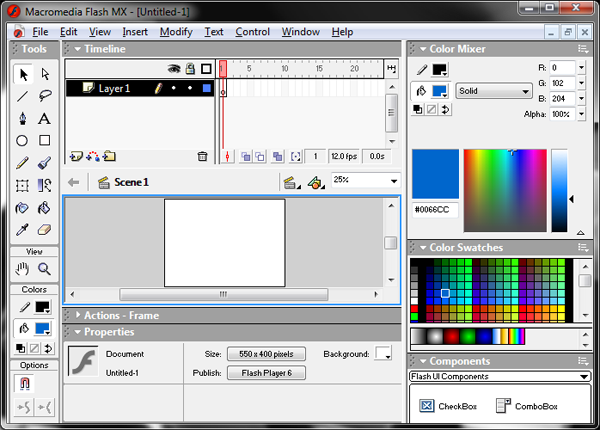
\includegraphics[width=0.8\textwidth]{./figures/flash-ui.png}
\caption{Prostředí programu Adobe Flash MX}
\label{fig:flash-ui}
\end{figure}



\subsection*{Vlastnosti}

Aplikace je volně ke stažení a~její použití je zdarma po získání bezplatné licence, k~vytváření aplikací je potřeba kromě prostředí znalost jazyka ActionScript\cite{ActionScript}, ve kterém se vytváří veškerá funkční logika. Projekt se musí nechat aplikací přeložit do souboru SWF\cite{swf}, který se potom vloží pomocí HTML\cite{html5video} elementu OBJECT na stránku. 

Prohlížeče návštěvníků stránky potom zavolají externí aplikaci, která tento SWF\cite{swf} soubor spustí a~zobrazí na stránce. Neřeší se pak v~tomto případě kompatibilní verze prohlížečů, ale verze externí apliace Adobe Flash\cite{flash}.

\begin{table}[h]\centering\footnotesize
	\caption[Kompatibilita Adobe FLash]{Kompatibilita Adobe Flash}\label{tab:research-flash}
	\begin{tabular}{|m{2.5cm}|m{2.5cm}|m{2.5cm}|m{2.5cm}|}\hline
		Internet Explorer & Gecko(Mozilla Firefox, Opera)	& WebKit (Safari, Google Chrome) &  Mobilní prohlížeče
		\tabularnewline \hline \hline 
		Ano od verze 6 &  Ano & Ano & Ne
		\tabularnewline \hline
	\end{tabular}
\end{table}


\subsection*{Zhodnocení}

Adobe Flash\cite{flash} je velmi rozšířený vzhledem k~velice bohatým možnostem interakce s~uživatelem a~zjednodušení pro testování mezi prohlížeči. Díky tomu je upředňostňovaný pro spoustu interakcí mezi uživateli. 

Hlavní nevýhoda je pak vysoká náročnost na výkon počítače, což se pak negativně projeví na výdrži baterie u~přenosných zařízení a~to i~u dobře optimalizované aplikace.  Další velkou nevýhodou je nedostatečná podpora v~mobilních zařízení\cite{mobile} v~dnešní době. 


\section{GIF}

GIF\cite{gif} je formát pro ukládání obrázků, který s~možností sekvence několika obrázků za sebou dokáže vytvořit animaci. V~průzkumu ho uvádím zejména pro to, že mnoho animací nebo krátkých videí se realizuje právě v~tomto formátu.

\subsection*{Vlastnosti}

Formát GIF\cite{gif} je používán pro grafiku s~malou paletou barev pro krátká videa nebo animace s~malým rozlišením. V~případě animace se ukládá každý krok v~animaci jako další obrázek. Kromě volby, zda se budou kroky animace opakovat nebo proběhnou pouze jednou, zde není žádná možnost ovládání. Grafika v~obrázku GIF je omezena na 256 barev, jedna z~nich je průhledná. Samotný obrázek je pak uložen bezztrátově, takže se často používá pro uložení jednoduše zbarvených firemních log.

\begin{table}[h]\centering\footnotesize
	\caption[Kompatibilita GIF]{Kompatibilita GIF}\label{tab:research-gif}
	\begin{tabular}{|m{2.5cm}|m{2.5cm}|m{2.5cm}|m{2.5cm}|}\hline
		Internet Explorer & Gecko(Mozilla Firefox, Opera)	& WebKit (Safari, Google Chrome) &  Mobilní prohlížeče
		\tabularnewline \hline \hline 
		Ano  &  Ano & Ano & Ano
		\tabularnewline \hline
	\end{tabular}
\end{table}

\subsection*{Zhodnocení}

Tento převážně obrázkový formát je málokdy používán k~nějakým ilustracím na webových stránkách. Je rozšířený hlavně kvůli jeho jednoduchosti při vytváření oproti jiným srovnávaným formátům. Návrh a~implementace této bakalářské práce dokáže formát GIF nahradit u~některých typových příkladů. 

Hlavní nevýhodou je omezené spektrum barev. Prohlížeče vykreslují GIF jako obrázek, takže se nedá nijak ovládat nebo nějak reagovat na uživatele. Naopak GIF formát je dostupný na všech používaných prohlížečích, takže se velice jednoduše integruje.


\section{HTML5 Video}

Moderní webové prohlížeče nám umožňují vkládat video přímo do prohlížeče. Tento způsob se používá pro přehrávání například na stránkách Youtube\cite{youtubeHtml5}. 
Video musí být uloženo v~přehratelném formátu MP4\cite{mp4}. Díky tomu prohlížeč dokáže začít přehrávat video nebo animaci, i~když ještě nemá stažený celý soubor.


\subsection*{Vlastnosti}

Video v~HTML5 se do webové stránky vkládá jako  HTML\cite{html5video} element, ve kterém se uvede cesta k~MP4\cite{mp4} souboru a~další parametry (například velikost objektu na stránce). Tento element je pak ve struktuře HTML, díky tomu aktivně dokáže komunikovat pomocí Javascriptu\cite{javascript}. To znamená, že se dá veškeré ovládání velice jednoduše řešit v~nativních knihovnách prohlížeče. 


\begin{table}[h]\centering\footnotesize
	\caption[Kompatibilita HTML5]{Kompatibilita HTML5 Video}\label{tab:research-html5}
	\begin{tabular}{|m{2.5cm}|m{2.5cm}|m{2.5cm}|m{2.5cm}|}\hline
		Internet Explorer & Gecko(Mozilla Firefox, Opera)	& WebKit (Safari, Google Chrome) &  Mobilní prohlížeče
		\tabularnewline \hline
		9.0+  &  Ano & Ano & Částečná (pouze režim přes celou obrazovku)
		\tabularnewline \hline
	\end{tabular}
\end{table}

\subsection*{Zhodnocení}

Tento formát je určen pro přehrávání videí a~filmů z~reálného prostředí. Animace na stránkách jsou předem připraveny digitálně. Problémem je funkčnost na mobilních zařízení, kde se HTML5 video přehrává na celé obrazovce\cite{html5VideoSupport}. Pokud nám jde pouze o~video, jeví se toto jako nejlepší cesta. 

Mnohdy je ale tato technologi používán jako grafické doplnění stránky\cite{effectHtml5}. Momentálně na mobilních zařízení často dochází k~nekorektnímu zobrazení nebo znepřístupnění webové stránky.

Pokud bychom pomocí HTML5 videa řešili některé animace, budeme postrádat průhlednost a~spoustu procesů pro přípravu videa. Tento formát není pro animace na stránkách určený.

\section{Zhodnocení}

Všechny formáty, které byly představeny, vypadají na první pohled dostačující, ale může se stát, že se požaduje na webových stránkách animace, která bude fungovat stejně v~IE8 nebo na mobilních zařízení. Pak by požadavkům nevyhovoval žádný z~jmenovaných formátů. 

\begin{table}[h]\centering\footnotesize
	\caption[analysisResult]{Zhodnocení současných formátů}\label{tab:research-result}
	\begin{tabular}{|l||m{2.5cm}|m{2.5cm}|m{2.5cm}|}
	\hline
		Formát & Ovladatelnost (Javascript) & Podpora mobilních zařízení & Minimální verze IE
		\tabularnewline \hline \hline 
		Adobe Flash  &  Ano & Ne & IE6+ \\ \hline
		HTML5 Video  &  Ano & Částečná & IE9+ \\ \hline
		GIF  &  Ne & Ano & Všechny současné
		\tabularnewline \hline
	\end{tabular}
\end{table}

Současné možnosti vytváření animací na webových stránkách jsou postačující pokud je možnost vynechat některý z~nepodporovaných požadavků v~tabulce \ref{tab:research-result}. 

V této práci je v~následujících kapitolách popsán a~vytvořen takový formát, aby splňoval všechny požadavky, které ostatní formáty nepodporují:

\begin{itemize}
\item Podpora prohlížečů od verze Internet Explorer 8+
\item Stejné chování na všech mobilních zařízení.
\item Podpora ovládání pomocí jazyka Javascript
\end{itemize}


\chapter{Analýza}


V této kapitole je provedena analýza požadavků a~podle ní je navržena architektura výsledné aplikace. 


\section{Požadavky}

\subsection{Nefunkční požadavky}

Výsledný způsob animace by měl splňovat níže uvedené podmínky.

\subsubsection*{Animace v~prostředí webového prohlížeče}

Důvodem vzniku práce bylo poskytnutí formátu animace ve webovém prostředí, které bude mít díky modernějším technologiím výhodu v~efektivitě a~rychlosti. Je tedy zřejmé, že musíme dodržet základní podmínku a~to podporu ve všech majoritních prohlížečích. Vše by mělo fungovat bez použití doplňků nebo rozšíření v~prohlížečích.

\subsubsection*{Podpora pro mobilní zařízení}

Důvodem tohoto požadavku je fakt, že existující řešení mají velice malou podporu na~mobilních zařízení. Adobe Flash\cite{flash} není podporovaný vůbec, HTML5 Video\cite{html5video} je možné přehrávat pouze v~režimu na celou obrazovku, čímž se animace vytrhne z~kontextu stránky a~zobrazení je tím pádem špatné.

\subsubsection*{Ovládání animace}

Tento požadavek opět souvisí s~tím, že animací chceme stránku ozdobit v~jednom určitém momentu. Je tedy třeba poskytnout vývojářům, kteří by chtěli animovat nějakou část stránky, základní ovládací prvky.


\subsubsection*{Snadná integrovatelnost}

Pro vývojáře musí být co nejjednodušší integrace pomocí přidaných skriptů a~návodů. Animace jsou nyní uloženy jako film, tudíž je potřeba vytvořit program, který dokáže z~filmu vytvořit námi požadovaný formát.

Pokud bychom se připravovali na tento formát už od začátku, měli bychom seznam obrázků, kde každý z~nich obsahuje jeden krok animace.

\subsection{Funkční požadavky}

\subsubsection*{Vlastnosti generovacího skriptu}

Animace se bude pouštět pomocí Javascript knihovny, uživatelé stránek budou používat už předem připravenou a~vygenerovanou verzi. Pro vývojáře bude připraven generovací skript do tohoto formátu v~jazyce Python\cite{python}.

\begin{itemize}
\item Ukládání ve formátu PNG
\item Vytvoření časové osy každé animace
\item Možnost vygenerovat animaci ze sekvence snímků
\item Možnost vygenerovat animaci z~GIF obrázku
\item Možnost vygenerovat animaci z~videa s~nastavením kvality.
\end{itemize}

\subsubsection*{Vlastnosti přehrávače}

Tyto vlastnosti bude mít Javascript přehrávač animací

\begin{itemize}
  \item Možnost spustit animaci v~cyklu stále za sebou
  \item Možnost spustit animaci do konce nebo nějakého snímku 
  \item Možnost zvolit rychlost přehrávání
  \item Možnost skočit v~animaci na určitý snímek
  
\end{itemize}

\section{Případy užití}

\subsection{Vytvoření animace}

Programátor by měl mít možnost si vytvořit animaci v~tomto formátu z~dostupných zdrojů. Bude se tedy jednat o~vytvoření animace z~obrázků GIF nebo sekvence obrázků (například dostupných od grafika). Dále bude možnost generovat animaci například z~videa zachycené obrazovky.

\subsection{Přehrávání animace ve webovém prohlížeči}

Animace by měla být přehrávána ve webovém rozhraní na všech důležitých prohlížečích. Musí být zajištěna jednoduchá implementace do webové stránky pro programátora a~snadná ovladatelnost přehrávání. 


\section{Architektura projektu}

Řešení tedy rozdělíme do dvou částí. První část bude generovací skript, který animaci připraví ze vstupních formátů, druhá část se pak bude pouštět v webovém prohlížeči uživatelských počítačů. Pro každou část se budou používat trochu jiné technologie, vzhledem k~účelu použití, proto mají dva různé návrhy a~implementace.





\chapter{Definice formátu animace}

V této kapitole je popsán postup a~algoritmus vytváření animace. Jedná se o~zjednodušený algoritmus, který v podobné podobě používá například formát APNG\cite{apngFrames}. 


\section{Popis formátu animace}

Nástroj pro generování animace má za úkol přeformátovat vstupní animaci z~různých zdrojů (GIF, .mp4, .jpg) do tohoto formátu. Celý princip je založený na~tom, že se mezi jednotlivými snímky mění pouze část vykreslovaného pole (viz obrázek \ref{fig:algdiffs}). My si budeme ukládat informace o~tomto fragmentu a~jeho obsah. Tyto data poté uložíme do dvou souborů, podle kterých se bude řídit přehrávání. V~následujícím textu si projdeme všechny úkony, které algoritmus vytváří.

\subsection*{Snímky animace}

Jednotlivé fragmenty ze snímků budeme ukládat do jednoho velkého obrázku, který se bude po částech zase vykreslovat při přehrávání. Musíme zajistit, aby byly fragmenty vždy pouze jednou, abychom zajistili minimální možnou velikost dat. 


\section{Algoritmus zakódování z~dostupných formátů}
\label{section:algencode}

Tato sekce dokumentuje celý algoritmus výpočtu animace. Rozdělení tohoto algoritmu do tříd je podrobně popsáno u~návrhového modelu. 

\subsection{Inicializace}
Algoritmus na~vstupu dostane množinu snímků animace reprezentovanými maticí obrázků. První snímek slouží jako počáteční stav. 

\begin{figure}[h]
\centering

\includegraphics[width=1\textwidth]{figures/alg-frames.png}
\caption{Snímky ukázkové animace}
\label{fig:algframes}
\end{figure}

Pro lepší porozumění použijeme animaci západu slunce, animace má pouze 4 snímky kvůli jednoduchosti, ale dokážeme na ní předvést veškeré operace, které algoritmus provádí.


\subsection{Rozdíly mezi snímky animace}
\label{section:algdiffsformat}

Algoritmus má tedy načtené snímky animace. Nyní prochází postupně snímek za snímkem a~sleduje změny oproti předchozímu snímku. Na následujícím obrázku vidíme změny znázorněny červeně.

\begin{figure}[h]
\centering

\includegraphics[width=1\textwidth]{figures/alg-diffs.png}
\caption{Rozdíly mezi snímky animace}
\label{fig:algdiffs}
\end{figure}


\subsection{Optimalizace rozdílů snímků}

Algoritmus zajišťuje, aby rozdíly mezi snímky se shlukly do větších bloků, kvůli ušetření režie následného přehrávání. Na následujícím obrázku lze vidět, že algoritmus dal dohromady paprsky slunce se samotným sluncem. Tyto jednotlivé části animace poskláda do jednoho velkého obrázku a~zapamatuje si pozici (obrázek \ref{fig:algdiffs}). 

\begin{figure}[h]
\centering

\includegraphics[width=1\textwidth]{figures/alg-simplify.png}
\caption{Optimalizace rozdílů snímků}
\label{fig:algsimplify}
\end{figure}
\FloatBarrier

\subsection{Zakódovaná animace}

Prvním souborem na výstupu je výsledná bitmapa, kterou program uloží ve formátu PNG (obrázek \ref{fig:algresult}). Informace o~průběhu animace a~nalezené jednotlivé rozdíly jsou pak uloženy v~druhém souboru.

\begin{figure}[h]
\centering

\includegraphics[height=200pt]{figures/alg-result.png}
\caption{Grafika odeslaná na výstup}
\label{fig:algresult}
\end{figure}


\section{Přehrávání}

Při přehrávání máme k~dispozici obrázek se všemi částmi animace (obrázek \ref{fig:algresult}) a~soubor s~meta informacemi. Tedy informacemi, kdy a~co se má zobrazit v~animaci. K~výše uvedenému obrázku například existuje soubor, který nese souřadnice co se má zobrazit v~aktuálním snímku (obrázek \ref{fig:algmetadata}).

Přehrávač potom postupně zobrazuje části obrázku podle daných informací. 

\begin{figure}[h]
\centering
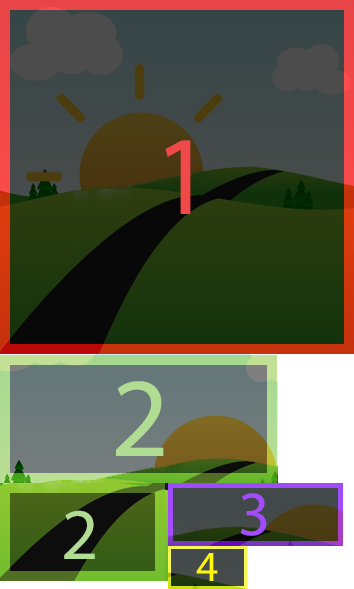
\includegraphics[height=200pt]{figures/alg-metadata.png}
\caption{Informace o~snímcích, které nese druhý soubor animace}
\label{fig:algmetadata}
\end{figure}



\chapter{Návrh generátoru animace}

\section{Návrhový model}

Vzhledem k~tomu, že tento program je určen pouze pro zpracování vstupu na~náš výstup a~neexistují žádné trvalé mezistavy, není vůbec použita databáze a~s tím spojený databázový model.

\begin{figure}[h]
\centering
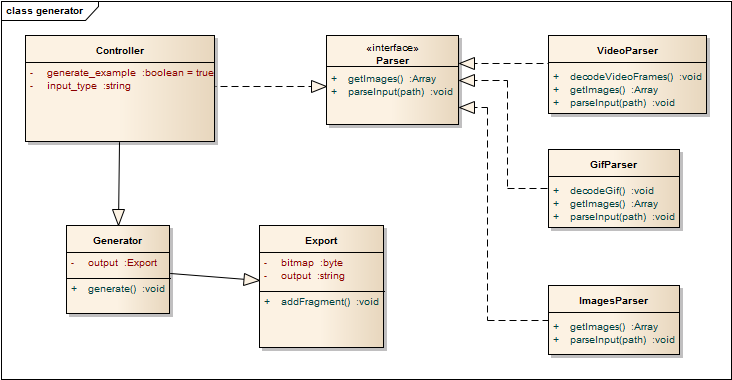
\includegraphics[width=1\textwidth]{figures/generator.png}
\caption{Návrhový model generátoru}
\label{fig:generator}
\end{figure}

\section{Popis tříd}

Následuje zde popis tříd generátoru animace. 

\subsection{Controller}
Controller je hlavní třída celého programu, která načítá všechny další služby pro správný běh programu. Stará se o~také o~kontrolu vstupu.

\subsection{Parser}
\label{secition:generatorparserclass}

Třídy, které implementují rozhraní Parser slouží k~načtení a~zpracování vstupu. Třída Controller načte vždy jen potřebný parser a~předá mu parametry pro načtení. Tato třída (resp. definovaná podtřída) převede vstup do unifikovaného formátu, který pak používá následující třída Generator. 

\subsection{Generator}

Tato třída obsahuje vlastní algoritmus pro vygenerování animace do našeho formátu, který je popsaný v~předchozí kapitole. Komunikuje s~výstupní třídou Exporter, kterému posílá výstupy.

\subsection{Exporter}

Třída Exporter se stará o~výstup aplikace. Vzhledem k~většímu počtu operací pro optimalizaci výstupu, zejména výstupu rastru velkého obrázku, je třeba tuto třídu definovat, nejedná se totiž pouze o~jednoduchý zápis do souboru. Stará se především o~minimalizaci výsledného formátu a~přidává přehrávací knihovnu.

\chapter{Implementace generátoru animace}

Tato kapitola je věnována implementaci generátoru a definovaného formátu animace z~předchozí kapitoly. Jedná se o~konzolovou aplikaci v~programovacím jazyku Python.

\section{Výběr programovacích jazyků}

Generátor bude fungovat jako aplikace běžící v~příkazovém řádku. Aplikace je určena především pro programátory, kteří jsou znalí tohoto prostředí. Pro napsání takové aplikace je možné použít řadu programovácích jazyků, z~nichž se nejvhodněji ukázal jazyk Python\cite{python}.

Python je implementován v~jazyce C\cite{c}. Charakterizuje se rychlostí, jelikož všechny kritické knihovny jsou implementovány právě v~jazyce C a~Python s~nimi velmi dobře komunikuje. Je například 3x - 5x rychlejší než jazyk PHP \cite{phpvspython}. Python není potřeba překládat do binární podoby, interpret spouští rovnou zdrojový kód, což vzhledem k~open-source povaze aplikace není problémem.  Python podporuje třídy, datové formáty a~další programátorské paradigmata objektového programování.

Dalším důvodem výběru tohoto jazyka je možnost použití knihovny Scipy\cite{Scipy}, která obsahuje několik algoritmických postupů, které použijeme při generování animace. 

Pro správný chod generátoru bude potřeba doinstalovat několik knihoven popsaných níže. Postup instalace je popsán v~Instalační příručce \ref{chapter:installation}.

\subsubsection*{Scipy}

Scipy je knihovna plná tříd a~objektů určená pro matematické výpočty, vědu nebo výzkum\cite{Scipy}. Je v~ní obsaženo velké množství funkcí včetně vykreslování grafů. Aplikace bude využívat její algoritmy nad velkým množství dat pro analýzu rozdílu jednotlivých kroků animace (kapitola \ref{section:genimpl})


\section{Postup vývoje}

Při vývoji bylo vyzkoušeno několik variant a~bylo nutno vyřešit určité problémy. Je důležité s~zmínit, že vlastní vývoj začal zejména až po definování formátu animace. V~následujícím seznamu je popsán přibližný harmonogram začátku vývoje.

\begin{itemize}
\item Získání dat z~několika obrázků, které tvoří snímky animace.
\item Nalezení rozdílů mezi těmito snímky
\item Export animace do námi vytvořeného formátu
\item Vytvoření jednoduchého přehrávače, který dokáže animaci přehrát
\end{itemize}

Po těchto úkonech bylo možné otestovat efektivitu tohoto formátu, z~čehož vznik první příklad popsaný v~sekci \ref{section:example1}. Jelikož byl formát efektivnější, pokračoval jsem v~implementaci dalších požadavků na obě části aplikace.

\subsection{Problémy}

Na úvod jsem se setkal hlavně s~problematickou kompatibilitou mezi verzemi Python 2.x a~3.x. Projekt je psaný v~jazyce Python verze 3.x, pro který není aktualizovaná spousta knihoven. To zpomalilo výběr knihovny pro porovnávání snímků animace.

Zjištění rozdílů mezi snímky a~jejich optimalizace je nakonec řešena díky knihovně Scipy.

\subsubsection*{Kompatibilita}

Vývoj probíhal na několika různých zařízeních. Při tom se objevilo množství problémů při instalaci knihoven, takže byla věnována zvláštní pozornost nastavení prostředí a~co nejjednoduššímu zprovoznění prostředí. 



\section{Realizace}
\label{section:genimpl}

Zde je popsaná adresářová struktura, která byla použita při realizaci generátoru. Byla navržena tak, aby vždy jeden soubor obsahoval jednu třídu nebo soubor podobných funkcí.


\begin{figure}[h]
    \dirtree{%
        .1 main.py\DTcomment{Spustitelný soubor generátoru}.
        .1 app.
        .2 controller.py\DTcomment{Třída Controller}.
        .2 generator.
        .3 generator.py\DTcomment{Třída Generator}.
        .2 parsers.
        .3 Interface.py\DTcomment{Rozhraní Parser}.
        .3 GifParser.py\DTcomment{Třída GifParser}.
        .3 VideoParser.py\DTcomment{Třída VideoParser}.
        .3 ImageParser.py\DTcomment{Třída ImageParser}.
        .2 export.
        .3 export.py\DTcomment{Třída Export}.
        .2 utils.
        .3 console.py\DTcomment{pomocné funkce pro výpis do konzole}.
    }
\end{figure}
\FloatBarrier


V následujících sekcích popíšu vybrané třídy, které mají zajímavou implementaci z pohledu implementace algoritmu zakódování animace.

\subsection{parsers/*}

Třídy dědící rozhraní \textbf{parsers/Interface.py} formátují vstup do námi potřebného formátu.

Pro vygenerování animačního formátu je potřeba definovat akceptované vstupní formáty. Vstup bude rozložen na~sekvenci po sobě jdoucích obrázků, které by vytvořily animaci. Tyto obrázky se budou načítat odlišně pro každý vstup. Tyto jednotlivé možnosti jsou zde rozepsány podle typu vstupu.

Vstupní metody pak načtou data do objektu \textbf{ndimage}, který poskytuje knihovna \textbf{Scipy}. Díky tomu bude možnost na snímcích animace provádět další operace.

\subsubsection*{parsers/ImageParser.py}

V této třídě se tedy pouze načtou obrázky ze složky na vstupu ve formátu \textbf{ndimage}.

Sekvence obrázků je jednoduchým vstupem. Na rozdíl od MP4 videa nebo formátu GIF zde jsou jednotlivé snímky samostatně vytvořené. Vstupem tedy bude složka s~očíslovanými obrázky. Vstupními parametry bude možné zadávat formát obrázku.

\subsubsection*{parsers/VideoParser.py}

Třída má za úkol zprocesovat data z~videa.

MP4 video je formát videa, ze kterého vytvoříme jednotlivé snímky podle zadaných vstupních parametrů - cesty k~videu a~intervalu mezi snímky. Externí knihovna ffmpeg\cite{videolib} pak vybere snímky z~videa podle intervalu. Dané snímky se pak převedou do formátu \textbf{ndimage}.

\subsubsection*{parsers/GifParser.py}

U GIF formátu bude podobný postup jako u~videa. Seznam snímků však vytváří knihovna PIL\cite{PIL} z~každého snímku z~GIF animace. Následné snímky převádí do potřebného formátu \textbf{ndimage}.

\subsection{generator/generator.py}

Pokud vstup proběhl bez problémů, je potřeba implementovat algoritmus pro zakódování animace (kapitola \ref{section:algencode}), čemuž odpovídá třída \textbf{Generator}.

V úvodu se obrázky rozdělí do dvojic - na obrázek první a~ten následující. Pak se pomocí funkce \textbf(find\_objects) najdou rozdíly mezi těmito dvěma obrázky, které jsou reprezentovány pomocí datové struktury \textbf{slice}. Toto pole se pak projde a~rozdíly, které mají k~sobě blízko se snaží sloučit na základě nějaké tolerované vzdálenosti.

Jakmile máme jsou tyto rozdíly hotové, seřadí se podle velikosti a~vytvoří se výsledný obrázek se všemy rozdíly mezi snímky. Tento obrázek a~informace o~snímcích se předají na výstup.


\subsection{export/export.py}

Celá animace je tvořena ze dvou souborů. Fragmenty animace se uloží do jednoho obrázku. Nejvhodnější je PNG formát vzhledem k~bezstrátové kompresi. Všechny rozdílné snímky animace jsou umístěné v~jednom obrázku, abychom snížili počet požadavků na~server. 

Druhým souborem jsou informace o~snímcích a~jejich použití. Tento soubor lze zakódovat do PNG obrázku díky jeho kompresi a~následné dekompresi při přehrání. Je ukládán ve formátu JSON. Jedná se o~formát, který slouží zejména pro přenos dat mezi serverem a~webovou aplikací a~tento princip bude používat i~vytvořený přehrávač. 

Výstup se řeší pomocí třídy \textbf{Export}, která nejdříve otestuje, zda je možný zápis do výstupní složky. Po vygenerování animace se pak uloží animace a~přidá se k~nim HTML šablona s~ukázkovým použitím.

\subsubsection*{Komprese výstupu}

Na výstupu se snažíme získat co nejmenší velikost kvůli datovým přenosům. Kompresi provedeme pomocí nástroje pngquant\cite{pngquant}, který optimalizuje barevné spektrum tak, byl výsledný obrázek pro lidské oko nerozeznatelný od původního nekomprimovaného souboru, ale měl přitom mnohem menší počet barev, což u~formátu PNG znamená menší velikost.

Soubor JSON můžeme zminimalizovat tak, že odstraníme přebytečné mezery a~tabulátory a~další nevýznamové znaky.

\section{Testování}

Interpret jazyka Python dokáže spustit i~kód, který například obsahuje přebytečné středníky, které jsem občas v~kódu psal ze zvyku z~jiných programovacích jazyků (C++, PHP). Pro zachování čistoty kódu je proto použit pylint\cite{pylint}, který zkontroluje veškeré nesrovnalosti v~kódu a~popřípadě vypíše chyby.

Jednotlivé části generátoru jsou testovány samostatně. Pro každou tuto část je napsaný jednotkový test, který otestuje její chování.

Testy jsou napsané pomocí frameworku Nose\cite{nose} a~vše je připraveno v~nástroji Make\cite{make}. Testy lze spustit následujícím příkazem.


\begin{lstlisting}
cd ./src/impl/generator/ && make test
\end{lstlisting}


\chapter{Návrh přehrávače animace}
\label{section:playerdraft}

V této kapitole je vysvětlen nástroj pro přehrávání animace. Nástroj je vzhledem k~požadavkům vytvořen v~jazyce Javascript.

\section{Vstup}

Vstupem budou dva vytvořené soubory z~generovacího nástroje. Tato aplikace pouze přehrává daný formát, takže je podstatně jednodušší, než generátor animace. 

\section{Návrhový model}

Celá knihovna je díky zjednodušenému přístupu k~jednotlivým elementům  díky knihovně jQuery realizována jako doplněk do této knihovny. Celý návrhový model bude vytvořený tak, aby mohl být doplňkem knihovny jQuery\cite{jqueryplugin}. 


\begin{figure}[h]
\centering
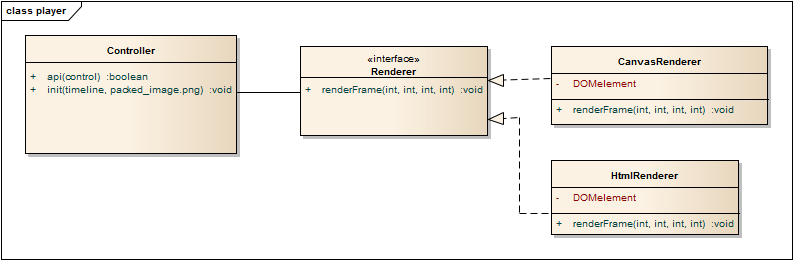
\includegraphics[width=1\textwidth]{figures/player.png}
\caption{Návrhový model knihovny}
\label{fig:player}
\end{figure}


\section{Popis tříd}

Zde je popsán návrhový model tříd knihovny pro přehrávání aplikace. 

\subsection{Controller}
Controller je hlavní třída celé knihovny pro přehrávání, která se stará o~načtení a~přijímá volání přes API. Ze vstupu a~na základě dalších faktorů vybere  správný renderer, který také ovládá. 

\subsection{Renderer}

Renderer je rozhraní, které se stará o~vykreslování animace. Podtřídy tohoto objektu se použijí podle možností prostředí prohlížeče. Na starých prohlížečích, které nepodporují HTML5, je potřeba zajistit zpětnou kompatibilitu (například IE6).

Objekt vykresluje podle souboru s~informacemi bitmapu v~prostředí prohlížeče. 

\chapter{Implementace přehrávače animace}


\section{Výběr jazyka a~programovacích knihoven}


V zadání a~požadavcích bylo stanoveno, že je potřeba dosáhnout použití v~nativních technologiích prohlížečů. Jediný skriptovací jazyk, který splňuje tuto podmínku je Javascript, takže výběr je omezený pouze na něj. Dále jsou použity některé nástroje a~knihovny, které pomáhají s~vývojem a~jsou popsány v~této sekci.

\subsubsection*{jQuery}

Pro Javascript existuje knihovna jQuery. Hlavní výhodou této knihovny je usnadnění práce s~DOM elementy a~jejich vlastnostmi mezi různými prohlížeči. Nemusíme se pak starat o~ošetření, v~jakém prohlížeči se momentálně nacházíme. Celý přehrávač bude implementován jako doplňek do tého knihovny, takže pro použití na stránkách bude potřeba mít tuto knihovnu implementovanou ve stránce. 

\subsubsection*{Grunt.js}

Při vývoji použijeme systém Grunt.js, který se bude starat o~automatizaci často opakovaných úkolů. Zejména se bude starat o~následující úkoly:


\begin{itemize}
  \item Optimalizace kódu Javascript a~vytvoření zmenšeného balíčku určeného k~nasazení 
  \item Testování aplikace
  \item Generování api dokumentace z~kódu
\end{itemize}

Upřesnění a~popis, jak se jednotlivé operace spouští, bude vysvětlen v~uživatelské příručce přehrávače \ref{chapter:documentation}.

\subsubsection*{Browserify}

Browserify je nástroj, pomocí kterého lze vytvořit jeden balíček z~více souborů. Díky tomuto nástroji je možné zdrojový kód přehledně skladovat v~několika souborech a~pomocí nástroje Grunt ho \"kompilovat\" do jednoho balíčku určeného k~použití. 



\section{Postup vývoje}

Vývoj probíhal ve dvou částech. Jakmile generátor vytvořil první validní výstup, byl vytvořen primitivní skript, který dokázal daný formát přehrát v~rámci webové stránky.

\subsection{Primitivní verze algoritmu}

Zmíněná primitivní verze měla za úkol pouze zobrazit definovaný formát a~zobrazit ho na webové stránce. Pro příklad je zde zobrazena testovací nejprimitivnější verze funkčního přehrávače.

\begin{figure}[h!]
\caption{Kód jednoduchého algoritmu pro vykreslení}
\begin{lstlisting}
<script type="text/javascript" src="anim_metadata.js"></script>
<canvas id="canvas" width="354" height="354"></canvas>
<script>
  var img = new Image();
  var _timeline = $.getJSON('anim_metadata.json')
  var ctx = document.getElementById("canvas").getContext('2d');
  img.onload = function()
  {
    var i = 0; // aktualni snimek, zaciname na 0
    var f = function() // funkce vykresli snimek
    {
      var frame = i++ % _timeline.length; // cislo snimku
      var parts = _timeline[frame].blit; // zmenene casti

      for (var j = 0; j < parts.length; ++j)
      {
        var part = parts[j]; // souradnice
        ctx.drawImage.apply( // vykresli zmenenou cast
          ctx,
          [img].concat(part).concat([part[2], part[3]])
        );
      }
      window.setTimeout(f, 500) // opakuj za dalsich 500ms
    };
    f(); // spust animaci
  };
  img.src = './anim_packed.png'; // nacist obrazek
</script>
\end{lstlisting}
\end{figure}
\FloatBarrier

V kódu, jak je vidět z~ukázky, se nejprve definuje vykreslující element a~načtou se metadata animace, tedy jeden ze souborů animace. V~Javascriptu se pak definuje, co se má stát při změně snímku, která je pevně definovaná každých 500ms. V~každé změně se změní části z~grafiky podle dat z~načteného souboru metadat. 


\subsection{Vývoj plnohodnotné verze}

Jakmile byl generátor animace, který spolupracoval správně s~tímto jednoduchým přehrávačem, hotov, začala práce na plnohodnotném přehrávači podle návrhu aplikace přehrávače definovaného v~kapitole \ref{section:playerdraft}. Nejprve bylo potřeba nastavit vývojové prostředí pomocí aplikace Grunt a~následně se vytvořil funkční přehrávač pro knihovnu jQuery. Implementace tříd a~komunikací mezi nimi proběhla bez větších problémů.

\subsubsection*{Implementace jako jQuery plugin}

Implementace jako jQuery pluginu byla jednoduchá. Kvůli jednoduchosti ovládání byl implementován postup, aby se instance přehrávače ukládala k~objektu. Výhodou tohoto přístupu je to, že si nemusíme ukládat instanci vytvořené animace pro pozdější kontrolu, ale můžeme ji získat opět z~daného objektu jako je ukázáno v~následující ukázce:

\begin{figure}[h]
\caption{Ukázka použití pluginu, když je uložen u elementu}
\begin{lstlisting}
  // v jedne casti aplikace
  $("#canvas").html5anim({
    src: 'animation/packed.png',
    timeline: 'animation/timeline.json'
  });

  ...

  // v jine casti aplikace
  $("#canvas").html5anim('pause');
\end{lstlisting}
\end{figure}

Celá dokumentace je podrobně popsána v~uživatelské příručce (příloha \ref{chapter:documentation}).

\section{Testování}

Javascriptový kód má kontrolovanou sémantičnost pomocí jslint\cite{jslint} tak, aby byla zajištěna přehlednost a~jednotnost kódu. Dále je otestováno veřejné API rozhraní výsledné animace pomocí nástroje Mocha\cite{mocha}.


\chapter{Ukázky aplikace}

V této kapitole jsou popsány 3 základní použití aplikace a~zhodnocení se vstupem. 

\section{Příklad: Převod GIF animace}
\label{section:example1}

V tomto příkladu si ukážeme převod animovaného obrázku ve formátu GIF do námi vytvořeného formátu. Zkusíme porovnat výsledek a~popsat výhody a~nevýhody. 

\subsection{Generování}

Animaci vygenerujeme následujícím příkazem. Vygenerovaný výsledek lze najít na přiloženém CD (/examples/01-gif/)

\begin{lstlisting}
$ src/impl/generator/main.py gif src/examples/gif/preloader.gif
Packing rectangles: 35 frames: 10
Packing finished took: 0.26485490798950195
Animation generated. Check out output path: ./generated
\end{lstlisting}

\subsection{Porovnání}

Výstup je vzhledově naprosto identický, změna je ve velikosti  souborů. Vstupní obrázek GIF (24Kb) je zredukovaný o~87.5\% na úctyhodné 3Kb. 

K tomu jako výhodu máme možnost ovládat výstup přes API přehrávače, tedy můžeme animaci zastavit nebo zrychlit. Výstupní formát je mnohem bohatší oproti obrázkům ve formátu GIF, které jsou omezeny na 256 barev, takže výstup je bezztrátový.

\subsection{Zhodnocení výstupu}

Z porovnání vidíme, že náš formát bez ztráty kvality ušetřil dostatek dat a~nám se konverze vyplatí. V~tomto příkladu jsme použili jednoduchou animaci, takže změnšení velikosti je významné. Na jiné a~složitější animaci (/examples/01b-gif) již není zmenšení datové velikosti tak razantní. V~obou případech je výhodou oproti klasickému formátu GIF ovladatelnost v~prohlížeči. 

\newpage
\section{Tapdaq  - Aktivace SDK}

V tomto případě bychom chtěli představit implementaci služby Tapdaq. Normálně by se daly použít klasické statické obrázky, ale s~tímto formátem můžeme jednotlivé obrázky rozhýbat.

Proto jsme si nahráli rychlý záznam z obrazovky implementace dané knihovny. Výsledný video soubor měl velikost 10.4 MB. 

\subsection{Generování}

Animaci jsme vygenerovali pomocí následujícího příkazu. Přidali jsme parameter v, který přidá více informací na výstup, abychom věděli, zda proces probíhá v~pořádku. Jak je uvedno v~následujícím výpisu, celý zabral necelých šest minut.

\begin{lstlisting}
$ src/impl/generator/main.py -v video src/examples/video/tapdaq.mov
Packing rectangles: 683 frames: 23
...
Packing finished took: 350.26485490798950195
Animation generated. Check out output path: ./generated
\end{lstlisting}

\subsection{Porovnání}

Animační formát jsme generovali z~videa nahraného v~počítači uživatele. Zdrojové video je plynulé a~kvaliní.

Vygenerovaná animace je mnohem více sekaná a~zrychlená. Je to dáno tím, že se bere pouze jeden snímek za sekundu. Námi vytvořená animace má stejnou kvalitu barev. Postrádá oproti videu jen plynulost.

\subsection{Zhodnocení výstupu}

Pokud bychom chtěli plynulé video, náš formát by byl neefektivní. Výsledná velikost je pouze 18\% z~originální velikosti. To je jednoznačně výhoda, ale v~tomto příkladu už vidíme ztrátu kvality. 

Další výhodou vygenerované animace je širší podpora. Zatímco u~zdrojového videa není úplná podpora (tabulka \ref{tab:research-html5}), vygenerovaný formát má podporu kompletní. 

Pokud nám nevadí znatelně menší kvalita videa, vygenerovaný formát nám pak přináší výhodu menší datové náročnosti a~širší podpory.

\newpage



\begin{conclusion}

Nový formát, který vznikl a~je zdokumentován v~této práci, slouží jako kvalitní alternativa formátu GIF. S~kompromisem dokáže nahradit i~HTML5 video na stránkách. 

Z definice algoritmu je zřejmé, že pro ukládání videa nebo animace, kde mezi snímky jsou velké rozdíly, tento formát nepřinese žádné výhody. Naopak výsledná animace by byla pravděpodobně větší. Ovšem například u~zobrazení průchodu aplikací je tento formát užitečný. 

Na práci bylo zajímavé kromě pouze návrhu a~implementace provádět výzkumnou část. Hlavní myšlenka už sice existovala, ale prozkoumat a~navrhnout generátor bylo zajímavé. Formát používám v~soukromých projektech a~v praxi se osvědčil již v~průběhu psaní této práce.


\section{Budoucnost}

V budoucnu bych chtěl zpřístupnit tento styl animace komunitě dalších programátorů. Jako další krok bych části této práce přeložil do angličtiny a~uveřejnil. Tím bych chtěl vyvolat nad tímto přístupem diskuzi a~názory jiných vývojářů a~podle toho se ubíral dál.

Z implementace je kandidátem pro změnu generátor animace, kde by bylo možné zoptimalizovat operace při vytváření velké bitmapy. Tyto operace, ač fungují dobře, mají zbytečnou složitost, která by se dala předejít například ukládáním dílčích výsledků. 


\end{conclusion}

\bibliographystyle{csn690}
\bibliography{ref}

\appendix

\chapter{Seznam použitých zkratek}
% \printglossaries
\begin{description}
	\item[JSON] JavaScript Object Notation
	\item[CSS] Cascading Style Sheets
	\item[HTML] HyperText Markup Language
	\item[GIF] The Graphics Interchange Format 
	\item[PNG] Portable Network Graphics 
	\item[IE] Internet Explorer
	\item[MP4] MPEG-4 Part 14
\end{description}

\chapter{Obsah přiloženého CD}

%upravte podle skutecnosti

\begin{figure}
	\dirtree{%
		.1 readme.md\DTcomment{stručný popis obsahu CD}.
		.1 examples.
		.2 01-gif\DTcomment{zdrojové kódy k~prvnímu příkladu užití}.
		.2 01b-gif\DTcomment{zdrojové kódy k~prvnímu příkladu užití}.
		.2 02-tapdaq\DTcomment{zdrojové kódy k~druhému příkladu užití}.
		.1 src.
		.2 impl\DTcomment{zdrojové kódy implementace}.
		.3 generator\DTcomment{zdrojové kódy generátoru animace}.
		.3 player\DTcomment{zdrojové kódy přehrávací knihovny}.
		.2 thesis\DTcomment{zdrojová forma práce ve formátu \LaTeX{}}.
		.1 text\DTcomment{text práce}.
		.2 thesis.pdf\DTcomment{text práce ve formátu PDF}.
		.2 thesis.ps\DTcomment{text práce ve formátu PS}.
	}
\end{figure}


\chapter{Dokumentace použití}
\label{chapter:documentation}

V této kapitole je popsáno používání tohoto formátu a~to ať už vygenerování aplikace z~různých zdrojů tak přehrávání a~ovládání animace. 

\section{Generování animace}

Animace je generována pomocí Python aplikace, která je popsaná v~páté kapitole. Skript se pouští v~příkazové řádce počítače se vstupními parametry. Skript si sám kontroluje vstup a~poskytne v~případě problémů rychlou nápovědu. V~příkladech je použita cesta z~kořenového adresáře přiloženého CD. 

\begin{lstlisting}
$./src/impl/generator/main.py
Usage:
    main.py [ -v -o PATH -s STEP] images <path>
    main.py [ -v -o PATH] video <file>
    main.py [ -v -o PATH] gif <file>
    main.py (-h | --help)
\end{lstlisting}


Ve výpisu vidíme na prvním řádku chybu, která nastala, dále následuje nápověda, která nám ukazuje možné použití generátoru a~formát jeho vstupu. Pokud se vstup nerozpozná nebo je prázdný, program nahlásí konkrétní chybu a~ukončí se.


\subsection{Import videa}

Pokud bychom chtěli importovat video, můžeme použít jednoduchou syntaxi jako v~tomto příkladu: 


\begin{lstlisting}
generator.py video /examples/video/src/video.mp4
Running video parser.
Using default delay: 1000ms.
Found 24 frames, starting conversion.
Output written in video.mp4/ folder. 
\end{lstlisting}

Generátor projde aplikací a~úspěšně provede všechny potřebné operace. Import videa navíc dokáže přijmout další parametr, který slouží k~určení délky kroku animace. Pokud není uveden na vstupu, vybere se výchozí hodnota. V~ukázce níže je zobrazen výstup s~vlastní vstupní hodnotou.

\begin{lstlisting}
generator.py video -s 400 /examples/video/src/video.mp4
Running video parser.
Usign animation step: 400ms.
Found 48 frames, starting conversion.
Output written in video.mp4/ folder.
\end{lstlisting}


\subsection{Import sekvence obrázků}

Tento import je nejtriviálnějším importem pro generátor, jelikož jeho jediná operace je načtení obrázků a~ošetření, zda všechny obrázky existují a~fungují správně. Jeho příkladné použití je zobrazeno níže.

\begin{lstlisting}
generator.py images /examples/images/src/
Running images parser.
Found 18 frames, starting conversion.
Output written in /examples/images/src/animation/ folder.
\end{lstlisting}

\subsection{Import GIF obrázku}

Dále import podporuje animaci z~GIF obrázku. Vstupní obrázek se rozloží na jednotlivé snímky animace a~pustí se algoritmus.

\begin{lstlisting}
generator.py gif /examples/gif/src/animation.gif
Running gif parser.
Found 6 frames, starting conversion.
Output written in /examples/gif/src/animation/ folder.
\end{lstlisting}

\section{Použití animace na webové stránce}

Přehrávání animace je popsáno v~jazyce JavaScript. Počítá se, že veškeré instalační podmínky jsou splněny a~tedy je možné používát knihovnu jQuery.

\subsection{Inicializace}

Nejprve je potřeba vložit náš plugin pro přehrávání na stránku. Tento kód vložíme až po inicializaci jQuery.

\begin{lstlisting}
  <script src="html5anim.min.js" async="true"></script>
\end{lstlisting}

Na stránce je dále nutné definovat HTML element, ve kterém bude probíhat animace. Stylizace tohoto elementu je mimo obsah této práce a~v~přílohách je použit nestylizovaný HTML tag:

\begin{lstlisting}
  <div id="animation"></div>
\end{lstlisting}

Inicializace samotné animace už probíhá v~jQuery jakožto samostatný plugin. Tento plugin se stará o~veškerou funkcionalitu dané aplikace a~dokáže také posílat a~přijímat příkazy pro ovládání.

\begin{lstlisting}
  $(document).ready(function(){
    var element = $("#animation");
    // inicializace animace
    element.html5anim({
      src: 'animation/packed.png',
      timeline: 'animation/timeline.json',
      loop: false,
      autoplay: false // zacit prehravat hned po spusteni?
    });
    //konec inicializace
  });
\end{lstlisting}

Jakmile je animace načtená, je možné ji začít ovládat přes následující příkazy. Počítá se s~provedením inicializace (kódu z~předchozího odstavce).

\begin{lstlisting}
// spusteni animace (zastavi se u~konce)
element.html5anim('play');

// zastaveni animace
element.html5anim('pause');

//prehrani na 43.  krok animace
element.html5anim('playTo', 43); 

//prehrani zpet na 0. krok animace
element.html5anim('rewindTo', 0);

\end{lstlisting}

Knihovna dále nabízí možnost informovat uživatele, pokud nastane nějaká událost. Podporují se následující události:

\begin{itemize}
\item onLoad - po načtení animace 
\item onPlay - vždy po spuštění animace
\item onStop - vždy po zastavení animace (i pokud dojede do konce) 
\item onFrame ( krok animace ) - vždy při přejití na snímek

\end{itemize}

Komunikace může probíhat načtením těchto proměnných při inicializaci nebo později při komunikaci s~knihovnou.

\begin{lstlisting}
var element = $("#animation");
// inicializace animace
element.html5anim({
  src: 'animation/packed.png',
  timeline: 'animation/timeline.json',
  autoplay: false, // zacni prehravat po nacteni
  onFrame: function(i){
    //co se stane pri vykresleni i-teho snimku
    window.console.log( "Prave probiha " + i + " krok animace" );
  },
  onStop: function(){
    //co se stane pri zastaveni
    window.console.log( "Zastaveni animace" );
  }
});

//pridani odposlechu udalosti po inicializaci
element.html5anim('onPlay', function(){
  window.console.log("Animace je spustena" );
});


\end{lstlisting}
\chapter{Instalační příručka}
\label{chapter:installation}

\section{Generování animace}

Pro generátor je potřeba mít nainstalovaný překladač pro jazyk Python (verze 3). Pokud se bude konvertovat video, je potřeba nainstalovat podpůrnou knihovnu ffmpeg\cite{videolib}. Další požadavky lze nainstalovat pomocí balíčkovacího systému \textbf{pip}\cite{pip}:

\begin{lstlisting}
make install
\end{lstlisting}

Pokud uživatel nemá nainstalovaný balíčkovací systém \textbf{pip}, seznam požadavků nalezne v~souboru requirements.txt:

\begin{lstlisting}
docopt==0.6.1
scipy
numpy
pillow
av
\end{lstlisting}

\newpage
\section{Knihovna pro přehrávání}

Knihovna pro přehrávání je, jak už je napsáno v~požadavcích, založena na technologiích, které poskytne samotný prohlížeč. Na webový prohlížeč jsou tím pádem minimální požadavky. 

\begin{itemize}
  \item Webový prohlížeč (podporované verze)
  \begin{itemize}  
  \item Firefox 4.0+ 
  \item Opera 6.0+
  \item Internet Explorer 8.0+
  \item  Safari 5+
  \item Google Chrome
  \end{itemize}
\end{itemize}

Přehrávání bude probíhat na webové stránce, která se generuje z~HTML kódu, na který jsou požadavky pro načtení souborů v ~následujícím seznamu.

\begin{itemize}
\item Knihovna jQuery, alespoň verze 1.9 (popř. 2.0+)
\end{itemize}


\end{document}
